\section{Casi d'uso}
\subsection{Attore}
Poiché per lo svolgimento del progetto non è necessario gestire permessi differenti per l'accesso alle funzionalità, l'attore che interagisce con il nostro software è unico, denominato "Utente".\\
\textbf{Utente:} soggetto che utilizza la web application, sfruttandone le funzionalità.
\subsection{UC1 - Visualizzazione lista dei dataset disponibili}
\begin{figure}[h!]
    \centering
    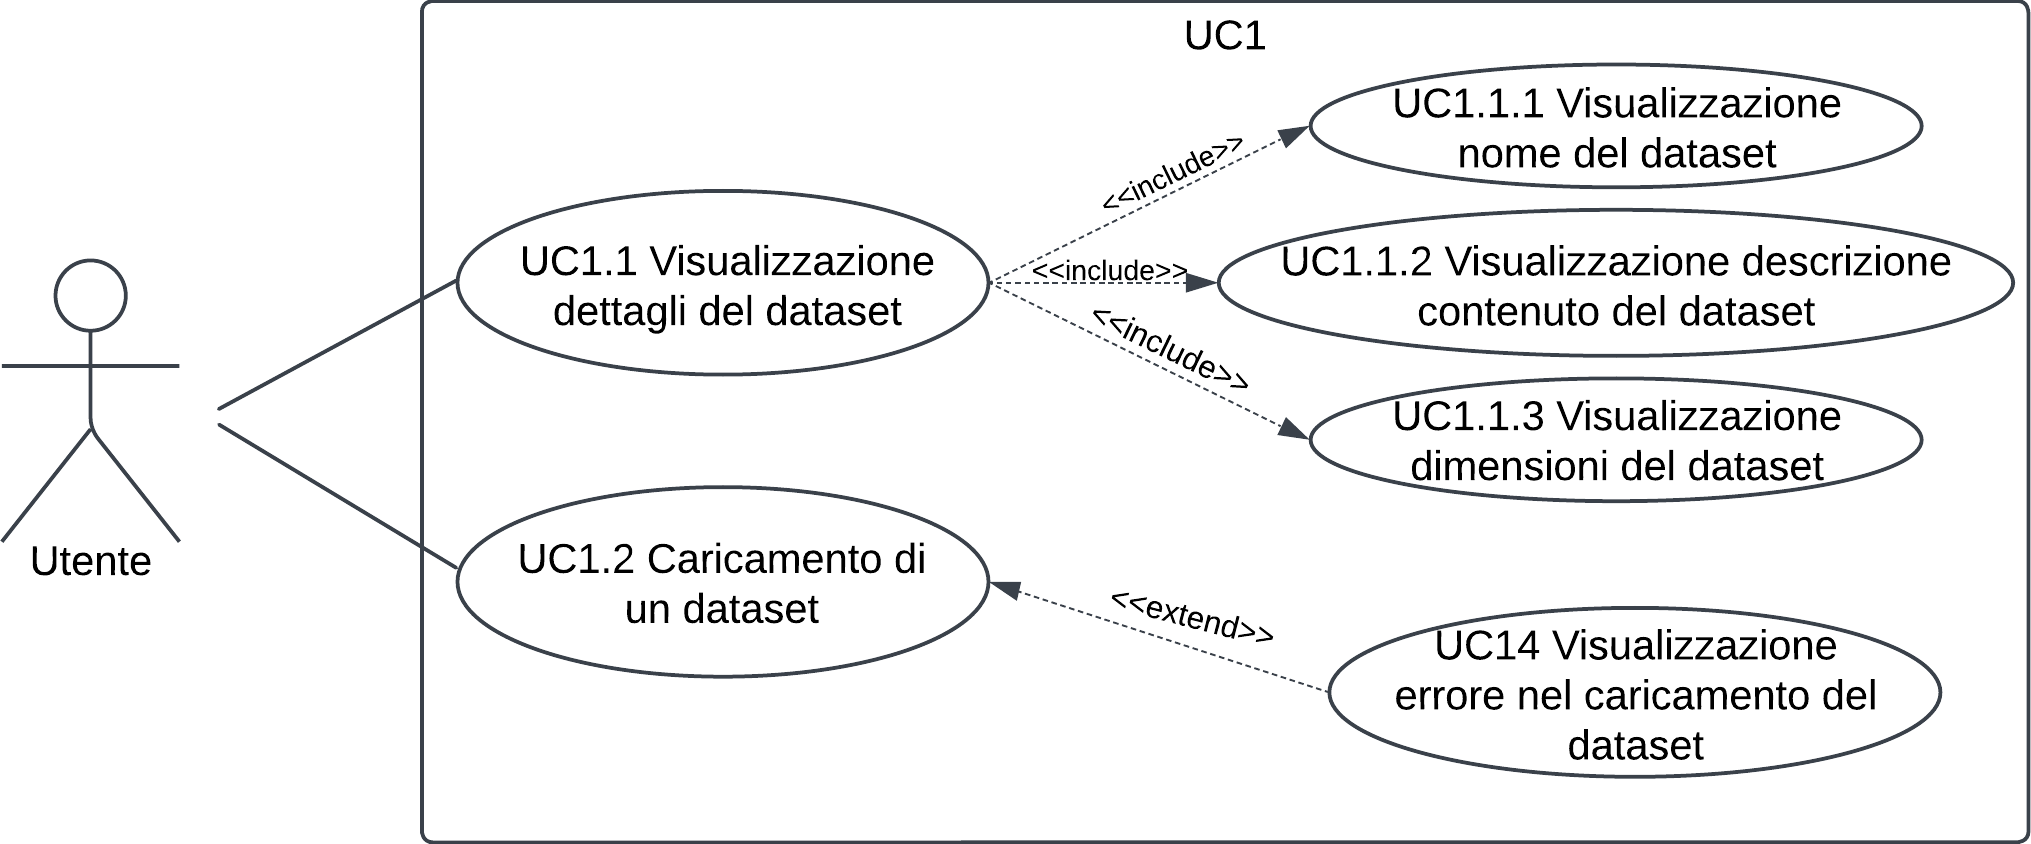
\includegraphics[scale=0.7]{template/images/UC1.png}
    \caption{UC1 - Visualizzazione lista dei dataset disponibili}
\end{figure}
\begin{itemize}
    \item \textbf{Attore:} utente;
    \item \textbf{Descrizione:} quando un utente interagisce con l'applicazione web,
    gli viene mostrato un elenco di dataset.\\ Da questa lista, può scegliere il dataset da rappresentare sotto forma di tabella e di grafico 3D.
    \item \textbf{Precondizioni:}
    \begin{itemize}
        \item L'utente ha accesso all'applicazione.
    \end{itemize}
    \item \textbf{Postcondizioni:}
    \begin{itemize}
        \item L'utente vede una lista dei dataset disponibili.
    \end{itemize}
    \item \textbf{Scenario:} 
    \begin{itemize}
        \item L'utente avvia il sistema;
        \item I dataset disponibili vengono presentati tramite un elenco;
        \item L'utente può navigare l'elenco e scegliere il dataset che gli interessa.
    \end{itemize}
\end{itemize}
\newpage
\subsubsection{UC1.1 - Visualizzazione dettagli del dataset}
\begin{itemize}
    \item \textbf{Attore:} utente;
    \item \textbf{Descrizione:} permette di visualizzare i dettagli del dataset selezionato;
    \item \textbf{Precondizioni:}
    \begin{itemize}
        \item Il sistema ha accesso ai dettagli tecnici e descrittivi del dataset.
    \end{itemize}
    \item \textbf{Postcondizioni:}
    \begin{itemize}
        \item Le informazioni sul dataset vengono mostrate all'utente.
    \end{itemize}
    \item \textbf{Scenario:}
    \begin{itemize}
        \item Il sistema mostra i dettagli dei dataset presenti nell'elenco.
    \end{itemize}
\end{itemize}
\paragraph{UC1.1.1 - Visualizzazione nome del dataset}
\begin{itemize}
    \item \textbf{Attore:} utente;
    \item \textbf{Descrizione:} l'utente può visualizzare il nome del dataset presente nell'elenco;
    \item \textbf{Precondizioni:}
    \begin{itemize}
        \item Il sistema ha accesso alle informazioni sul dataset.
    \end{itemize}
    \item \textbf{Postcondizioni:}
    \begin{itemize}
        \item Il nome del dataset viene mostrato all'utente.
    \end{itemize}
    \item \textbf{Scenario:}
    \begin{itemize}
        \item Il sistema mostra il nome del dataset.
    \end{itemize}
\end{itemize}
\paragraph{UC1.1.2 - Visualizzazione della descrizione contenuto del dataset}
\begin{itemize}
    \item \textbf{Attore:} utente;
    \item \textbf{Descrizione:} l'utente può visualizzare una descrizione del contenuto del dataset;
    \item \textbf{Precondizioni:}
    \begin{itemize}
        \item Il sistema ha accesso alle informazioni relative al contenuto del dataset.
    \end{itemize}
    \item \textbf{Postcondizioni:}
    \begin{itemize}
        \item La descrizione del contenuto del dataset viene mostrata all'utente.
    \end{itemize}
    \item \textbf{Scenario:}
    \begin{itemize}
        \item Il sistema mostra una descrizione del contenuto del dataset.
    \end{itemize}
\end{itemize}
\paragraph{UC1.1.3 - Visualizzazione dimensioni tabella}
\begin{itemize}
    \item \textbf{Attore:} utente;
    \item \textbf{Descrizione:} l'utente può visualizzare le dimensioni della tabella relativa ai dati contenuti nel dataset;
    \item \textbf{Precondizioni:}
    \begin{itemize}
        \item Il sistema ha accesso alle informazioni relative alla dimensione del dataset.
    \end{itemize}
    \item \textbf{Postcondizioni:}
    \begin{itemize}
        \item Le dimensioni della tabella relativa ai dati contenuti nel dataset vengono mostrate all'utente.
    \end{itemize}
    \item \textbf{Scenario:}
    \begin{itemize}
        \item Il sistema mostra le dimensioni della tabella relativa ai dati contenuti nel dataset.
    \end{itemize}
\end{itemize}

\subsubsection{UC1.2 - Caricamento di un dataset dall'elenco di quelli disponibili}
\begin{itemize}
    \item \textbf{Attore:} utente;
    \item \textbf{Descrizione:} consente di caricare il dataset selezionato nell'ambiente 3D dell'applicazione;
    \item \textbf{Precondizioni:}
    \begin{itemize}
        \item L'elenco dei dataset disponibili è stato caricato correttamente;
    \end{itemize}
    \item \textbf{Postcondizioni:}
    \begin{itemize}
        \item Il dataset selezionato viene caricato nel sistema.
    \end{itemize}
    \item \textbf{Scenario:}
    \begin{itemize}
        \item L'utente seleziona un dataset dall'elenco disponibile;
        \item Il sistema prepara i dati per la visualizzazione in forma tabellare e in grafico 3D.
    \end{itemize}
\end{itemize}
\newpage
\subsection{UC2 - Visualizzazione dati in forma tabellare}
\begin{figure}[h!]
    \centering
    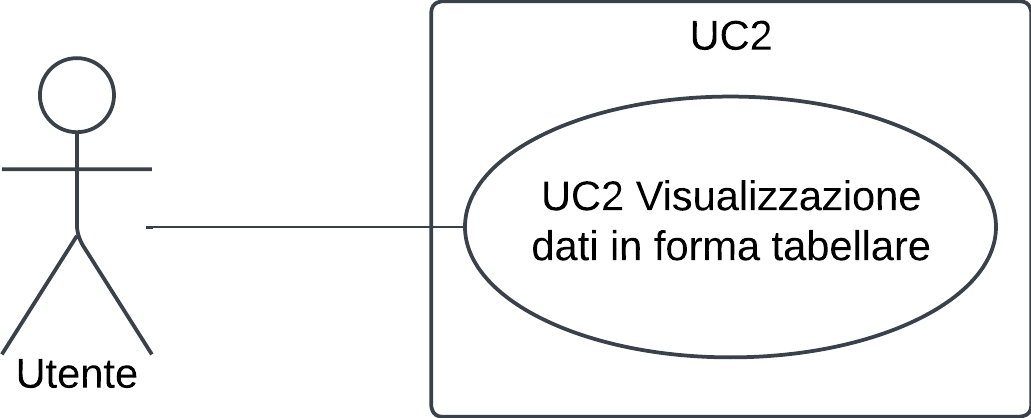
\includegraphics[scale=0.7]{template/images/UC2.png}
    \caption{UC2 - Visualizzazione dati in forma tabellare}
\end{figure}
\begin{itemize}
    \item \textbf{Attore:} utente;
    \item \textbf{Descrizione:} consente di visualizzare il dataset caricato sotto forma di tabella;
    \item \textbf{Precondizioni:}
    \begin{itemize}
        \item Il dataset selezionato è stato caricato correttamente.
    \end{itemize}
    \item \textbf{Postcondizioni:}
    \begin{itemize}
        \item I dati sono mostrati in forma tabellare.
    \end{itemize}
    \item \textbf{Scenario:}
    \begin{itemize}
        \item Il dataset selezionato viene caricato correttamente;
        \item L'applicazione elabora i dati e vengono mostrati in forma tabellare.
    \end{itemize}
\end{itemize}
\subsection{UC3 - Visualizzazione dati in forma di grafico a istogramma 3D verticale}
\begin{figure}[h!]
    \centering
    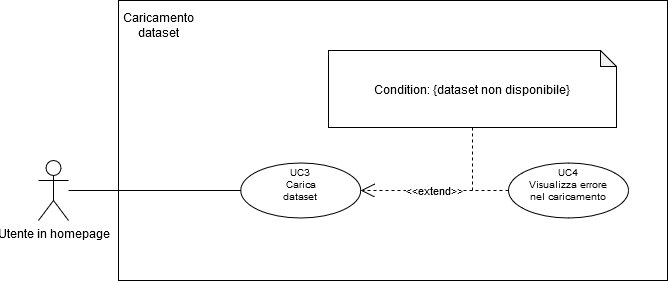
\includegraphics[scale=0.7]{template/images/UC3.png}
    \caption{UC3 - Visualizzazione dati in forma di grafico a istogramma 3D verticale}
\end{figure}
\begin{itemize}
    \item \textbf{Attore:} utente;
    \item \textbf{Descrizione:} consente di visualizzare il dataset caricato sotto forma di grafico a istogramma 3D verticale;
    \item \textbf{Precondizioni:}
    \begin{itemize}
        \item Il dataset selezionato è stato caricato correttamente.
    \end{itemize}
    \item \textbf{Postcondizioni:}
    \begin{itemize}
        \item I dati sono mostrati in forma di grafico a istogramma 3D verticale.
    \end{itemize}
    \item \textbf{Scenario:}
    \begin{itemize}
        \item Il dataset viene caricato correttamente;
        \item L'applicazione elabora i dati e viene creato un grafico a istogramma 3D verticale;
        \item L'interfaccia visualizza il grafico 3D verticale in una vista interattiva, consentendo all'utente di analizzare i dati.
    \end{itemize}
\end{itemize}
\subsection{UC4 - Visualizzazione assi}
\begin{itemize}
    \item \textbf{Attore:} utente;
    \item \textbf{Descrizione:} consente di visualizzare dettagliatamente gli assi X, Y e Z del grafico;
    \item \textbf{Precondizioni:} 
    \begin{itemize}
        \item Il grafico 3D è stato generato correttamente;
        \item Gli assi sono correttamente configurati nel sistema.
    \end{itemize}
    \item \textbf{Postcondizioni:}
    \begin{itemize}
        \item Gli assi X, Y e Z sono visibili e ben etichettati.
    \end{itemize}
    \item \textbf{Scenario:}
    \begin{itemize}
        \item L'utente visualizza il grafico 3D;
        \item L'utente visualizza gli assi X,Y e Z.
    \end{itemize}

\end{itemize}
\subsubsection{UC4.1 - Visualizzazione asse X}
\begin{itemize}
    \item \textbf{Attore:} utente;
    \item \textbf{Descrizione:} consente di visualizzare dettagliatamente l'asse X;
    \item \textbf{Precondizioni:} 
    \begin{itemize}
        \item L'asse X è configurato nel grafico.
    \end{itemize}
    \item \textbf{Postcondizioni:} 
    \begin{itemize}
        \item L'asse X è visibile e mostra i valori appropriati.
    \end{itemize}
    \item \textbf{Scenario:} 
    \begin{itemize}
        \item L'utente visualizza il grafico 3D;
        \item L'utente visualizza l'asse X con i valori appropriati.
    \end{itemize}
\end{itemize}
\subsubsection{UC4.2 - Visualizzazione asse Y}
\begin{itemize}
    \item \textbf{Attore:} utente;
    \item \textbf{Descrizione:} consente di visualizzare dettagliatamente l'asse Y;
    \item \textbf{Precondizioni:} 
    \begin{itemize}
        \item L'asse Y è configurato nel grafico.
    \end{itemize}
    \item \textbf{Postcondizioni:} 
    \begin{itemize}
        \item L'asse Y è visibile e mostra i valori appropriati.
    \end{itemize}
    \item \textbf{Scenario:} 
    \begin{itemize}
        \item L'utente visualizza il grafico 3D;
        \item L'utente visualizza l'asse Y con i valori appropriati.
    \end{itemize}
\end{itemize}
\subsubsection{UC4.3 - Visualizzazione asse Z}
\begin{itemize}
    \item \textbf{Attore:} utente;
    \item \textbf{Descrizione:} consente di visualizzare dettagliatamente l'asse Z;
    \item \textbf{Precondizioni:} 
    \begin{itemize}
        \item L'asse Z è configurato nel grafico.
    \end{itemize}
    \item \textbf{Postcondizioni:} 
    \begin{itemize}
        \item L'asse Z è visibile e mostra i valori appropriati.
    \end{itemize}
    \item \textbf{Scenario:} 
    \begin{itemize}
        \item L'utente visualizza il grafico 3D;
        \item L'utente visualizza l'asse Z con i valori appropriati.
    \end{itemize}
\end{itemize}
\subsection{UC5 - Visualizzazione legenda}
\begin{itemize}
    \item \textbf{Attore:} utente;
    \item \textbf{Descrizione:} consente di visualizzare una legenda con dettagli e informazioni sul grafico;
    \item \textbf{Precondizioni:} 
    \begin{itemize}
        \item Il grafico 3D è stato generato correttamente;
        \item Il sistema dispone delle informazioni necessarie per creare una legenda.
    \end{itemize}
    \item \textbf{Postcondizioni:}
    \begin{itemize}
        \item La legenda è visibile e fornisce informazioni dettagliate che aiutano l'utente a comprendere i dati rappresentati.
    \end{itemize}
    \item \textbf{Scenario:} 
    \begin{itemize}
        \item Il grafico viene generato correttamente;
        \item La legenda relativa al grafico è visibile.
    \end{itemize}
\end{itemize}
\subsection{UC6 - Pan}
\begin{figure}[h!]
    \centering
    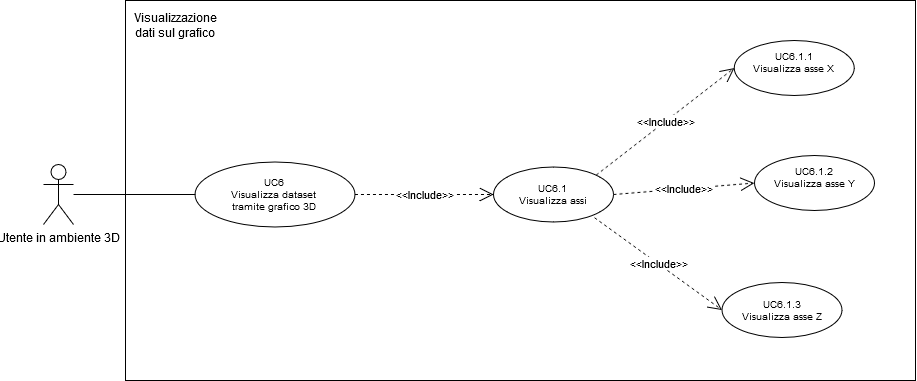
\includegraphics[scale=0.7]{template/images/UC6.png}
    \caption{UC6 - PAN}
\end{figure}
\begin{itemize}
    \item \textbf{Attore:} utente;
    \item \textbf{Descrizione:} l'utente sposta la visualizzazione del grafico 3D lungo il piano XY senza modificare l'orientamento della camera;
    \item \textbf{Precondizioni:}
    \begin{itemize}
        \item L'utente sta visualizzando il grafico 3D;
        \item Il sistema ha abilitato la funzionalità di interazione pan.
    \end{itemize}
    \item \textbf{Postcondizioni}:
    \begin{itemize}
        \item La vista della scena 3D è stata spostata nella direzione indicata dall'utente.
    \end{itemize}
    \item \textbf{Scenario:}
    \begin{itemize}
        \item L'utente visualizza il grafico 3D nell'interfaccia;
        \item L'utente interagisce con il grafico utilizzando il mouse (trascinamento);
        \item Il sistema interpreta il comando di spostamento e aggiorna la posizione del grafico lungo il piano XY;
        \item La nuova vista viene aggiornata in tempo reale e mostrata all'utente.
    \end{itemize}
\end{itemize}
\subsection{UC7 - Rotazione camera}
\begin{figure}[h!]
    \centering
    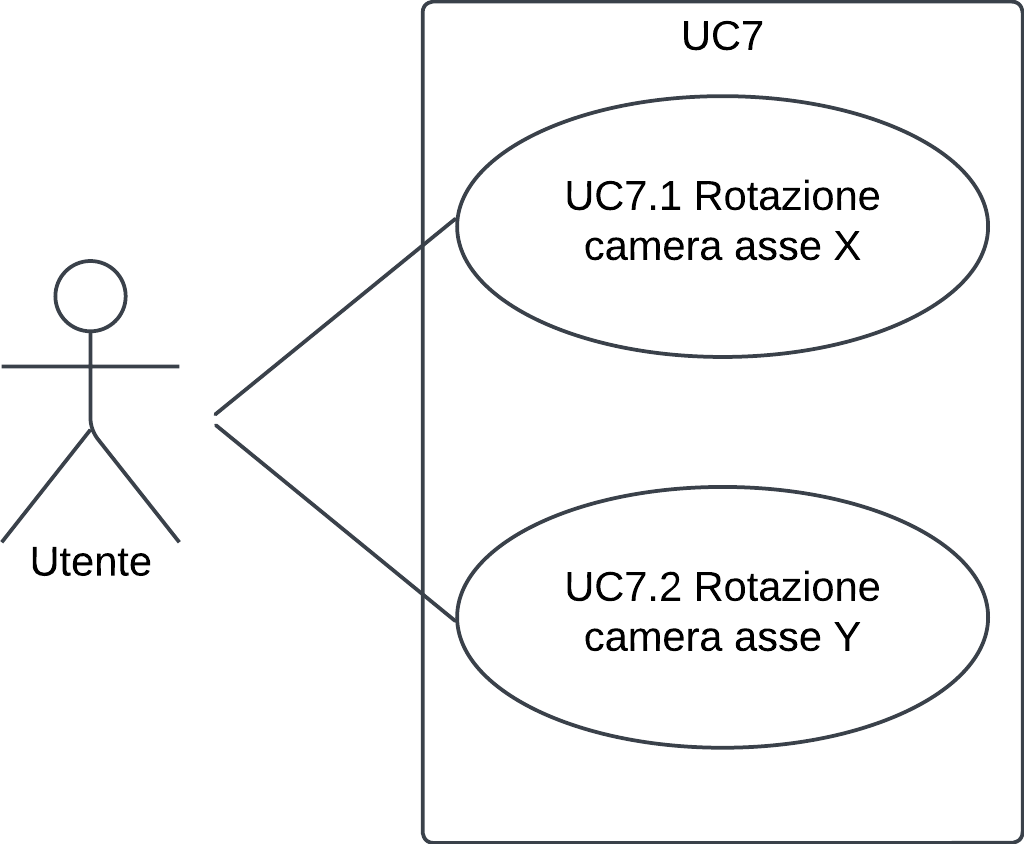
\includegraphics[scale=0.7]{template/images/UC7_7.1_7.2.png}
    \caption{UC7 - Rotazione camera}
\end{figure}
\begin{itemize}
    \item \textbf{Attore:} utente;
    \item \textbf{Descrizione:} l'utente ruota la visualizzazione del grafico 3D modificando l'orientamento della camera lungo uno o più assi. La rotazione consente di analizzare il grafico da diverse angolazioni;
    \item \textbf{Precondizioni:} 
    \begin{itemize}
        \item L'utente sta visualizzando il grafico 3D nell'interfaccia;
        \item Il sistema ha abilitato le funzionalità di interazione con la camera.
    \end{itemize}
    \item \textbf{Postcondizioni:} 
    \begin{itemize}
        \item La visualizzazione del grafico è stata aggiornata in base alla rotazione effettuata dall'utente.
    \end{itemize}
    \item \textbf{Scenario:} 
    \begin{itemize}
        \item L'utente interagisce con il grafico 3D usando i comandi per ruotare la visualizzazione. Il sistema aggiorna in tempo reale l'orientamento della camera, mostrando il grafico da una nuova angolazione.
    \end{itemize}
    
\end{itemize}
\subsubsection{UC7.1 - Rotazione camera asse X}
\begin{itemize}
    \item \textbf{Attore:} utente;
    \item \textbf{Descrizione:} l'utente ruota la visualizzazione del grafico 3D attorno all'asse X, modificando l'altezza della prospettiva.
    \item \textbf{Precondizioni:} 
    \begin{itemize}
        \item L'utente sta visualizzando il grafico 3D nell'interfaccia;
        \item Il sistema ha abilitato le funzionalità di interazione con la camera.
    \end{itemize}
    \item \textbf{Postcondizioni:} 
    \begin{itemize}
        \item La camera è stata ruotata attorno all'asse X, aggiornando la vista in tempo reale.
    \end{itemize}
    \item \textbf{Scenario:}
    \begin{itemize}
        \item L'utente usa comandi per spostare la vista verso l'alto o verso il basso. Il sistema ruota la camera attorno all'asse X, consentendo di osservare il grafico da un'angolazione più alta o più bassa.
    \end{itemize}
    
\end{itemize}
\subsubsection{UC7.2 - Rotazione camera asse Y}
\begin{itemize}
    \item \textbf{Attore:} utente;
    \item \textbf{Descrizione:} l'utente ruota la visualizzazione del grafico 3D attorno all'asse Y, modificando l'orientamento laterale della prospettiva;
    \item \textbf{Precondizioni:} 
    \begin{itemize}
        \item L'utente sta visualizzando il grafico 3D nell'interfaccia;
        \item Il sistema ha abilitato le funzionalità di interazione con la camera.
    \end{itemize}
    \item \textbf{Postcondizioni:} 
    \begin{itemize}
        \item La camera è stata ruotata attorno all'asse Y, aggiornando la vista in tempo reale.
    \end{itemize}
    \item \textbf{Scenario:} 
    \begin{itemize}
        \item L'utente usa comandi per spostare la vista verso destra o sinistra. Il sistema ruota la camera attorno all'asse Y, consentendo di osservare il grafico da angolazioni diverse lateralmente.
    \end{itemize}
\end{itemize}

\subsection{UC8 - Movimenti direzionali}
\begin{figure}[h!]\centering
    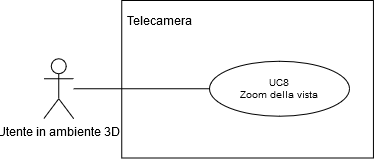
\includegraphics[scale=0.7]{template/images/UC8.png}
    \caption{UC8 - Movimenti direzionali}
\end{figure}
\begin{itemize}    
    \item \textbf{Attore:} utente;
    \item \textbf{Descrizione:} Compiere movimenti direzionali significa che, in ambiente di visualizzazione del grafico 3D, l'utente può interagire con il grafico compiendo degli spostamenti lungo i tre assi principali tramite comandi opportuni.
    \item \textbf{Precondizioni:}    
        \begin{itemize}
            \item Il caricamento del dataset è avvenuto con successo;
            \item La generazione dell'ambiente 3D e del relativo grafico non hanno riscontrato errori;
            \item Vengono eseguiti i comandi opportuni per i vari spostamenti.
        \end{itemize}    
    \item \textbf{Postcondizioni:}
        \begin{itemize}
            \item La telecamera che inquadra il grafico nell'ambiente 3D si troverà in una posizione diversa da quella in cui si trovava prima di compiere lo spostamento.
        \end{itemize}    
    \item \textbf{Scenario:} 
        \begin{itemize}
            \item L'utente interagisce con l'ambiente 3D per compiere un movimento direzionale.
        \end{itemize}
\end{itemize}
\subsubsection{UC8.1 - Movimento direzionale asse X}
\begin{itemize}    
    \item \textbf{Attore:} utente;
    \item \textbf{Descrizione:} L'utente interagisce opportunamente con l'ambiente 3D per spostarsi lungo l'asse X.
    \item \textbf{Precondizioni:}    
        \begin{itemize}
            \item Il caricamento del dataset è avvenuto con successo;
            \item La generazione dell'ambiente 3D e del relativo grafico non hanno riscontrato errori;
            \item Vengono eseguiti i comandi opportuni per lo spostamento lungo l'asse X.
        \end{itemize}    
    \item \textbf{Postcondizioni:}
        \begin{itemize}
            \item La telecamera che inquadra il grafico nell'ambiente 3D si troverà in una posizione diversa da quella in cui si trovava prima di compiere lo spostamento rispetto all'asse X.
        \end{itemize}    
    \item \textbf{Scenario:} 
        \begin{itemize}
            \item L'utente interagisce con l'ambiente 3D per compiere un movimento direzionale lungo l'asse X.
        \end{itemize}
\end{itemize}
\subsubsection{UC8.2 - Movimento direzionale asse Y}
\begin{itemize}    
    \item \textbf{Attore:} utente;
    \item \textbf{Descrizione:} L'utente interagisce opportunamente con l'ambiente 3D per spostarsi lungo l'asse Y.
    \item \textbf{Precondizioni:}   
        \begin{itemize}
            \item Il caricamento del dataset è avvenuto con successo;
            \item La generazione dell'ambiente 3D e del relativo grafico non hanno riscontrato errori;
            \item Vengono eseguiti i comandi opportuni per lo spostamento lungo l'asse Y.
        \end{itemize}    
    \item \textbf{Postcondizioni:}
        \begin{itemize}
            \item La telecamera che inquadra il grafico nell'ambiente 3D si troverà in una posizione diversa da quella in cui si trovava prima di compiere lo spostamento rispetto all'asse Y.
        \end{itemize}    
    \item \textbf{Scenario:} 
        \begin{itemize}
            \item L'utente interagisce con l'ambiente 3D per compiere un movimento direzionale lungo l'asse Y.
        \end{itemize}
\end{itemize}
\subsubsection{UC8.3 - Movimento direzionale asse Z}
\begin{itemize}    
    \item \textbf{Attore:} utente;
    \item \textbf{Descrizione:} L'utente interagisce opportunamente con l'ambiente 3D per spostarsi lungo l'asse Z.
    \item \textbf{Precondizioni:}    
        \begin{itemize}
            \item Il caricamento del dataset è avvenuto con successo;
            \item La generazione dell'ambiente 3D e del relativo grafico non hanno riscontrato errori;
            \item Vengono eseguiti i comandi opportuni per lo spostamento lungo l'asse Z.
        \end{itemize}    
    \item \textbf{Postcondizioni:}
        \begin{itemize}
            \item La telecamera che inquadra il grafico nell'ambiente 3D si troverà in una posizione diversa da quella in cui si trovava prima di compiere lo spostamento rispetto all'asse Z.
        \end{itemize}    
    \item \textbf{Scenario:} 
        \begin{itemize}
            \item L'utente interagisce con l'ambiente 3D per compiere un movimento direzionale lungo l'asse Z.
        \end{itemize}
\end{itemize}

\subsection{UC9 - Riposizionamento iniziale}
\begin{figure}[h!]\centering
    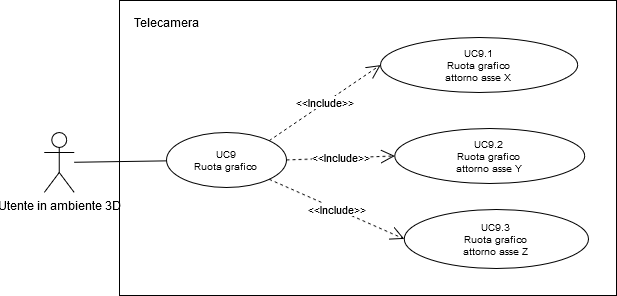
\includegraphics[scale=0.7]{template/images/UC9.png}
    \caption{UC9 - Riposizionamento iniziale}
\end{figure}
\begin{itemize}    
    \item \textbf{Attore:} utente;
    \item \textbf{Descrizione:} Riposizionare inizialmente la telecamera significa ripristinare la sua posizione e angolazione alla configurazione di partenza, annullando qualsiasi modifica apportata successivamente all'inizializzazione dell'ambiente 3D.
    \item \textbf{Precondizioni:}    
        \begin{itemize}
            \item Il caricamento del dataset è avvenuto con successo;
            \item La generazione dell'ambiente 3D e del relativo grafico non hanno riscontrato errori;
            \item Viene eseguito il comando opportuno per il riposizionamento iniziale.
        \end{itemize}    
    \item \textbf{Postcondizioni:}
        \begin{itemize}
            \item La posizione e angolazione della telecamera corrispondono alla configurazione di iniziale, uguale a quella di inizializzazione dell'ambiente 3D.
        \end{itemize}    
    \item \textbf{Scenario:} 
        \begin{itemize}
            \item L'utente interagisce con l'interfaccia per ripristinare la posizione e angolazione della telecamera ai valori iniziali.
        \end{itemize}
\end{itemize}

\subsection{UC10 - Visualizzazione dei valori di una barra del grafico}
\begin{figure}[h!]\centering
    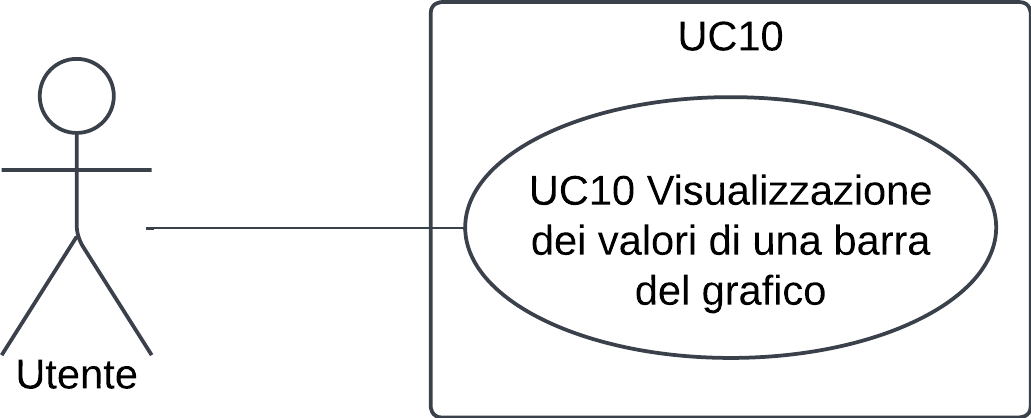
\includegraphics[scale=0.7]{template/images/UC10.png}
    \caption{UC10 - Visualizzazione dei valori di una barra del grafico}
\end{figure}
\begin{itemize}    
    \item \textbf{Attore:} utente;
    \item \textbf{Descrizione:} L'utente, tramite interazione opportuna, può selezionare una barra del grafico all'interno dell'ambiente 3D per visualizzarne i rispettivi valori.
    \item \textbf{Precondizioni:}    
        \begin{itemize}
            \item Il caricamento del dataset è avvenuto con successo;
            \item La generazione dell'ambiente 3D e del relativo grafico non hanno riscontrato errori;
            \item Viene eseguita l'interazione opportuna da parte dell'utente per la selezione della barra del grafico.
        \end{itemize}    
    \item \textbf{Postcondizioni:}
        \begin{itemize}
            \item Vengono visualizzati a schermo i valori della barra del grafico selezionata.
        \end{itemize}    
    \item \textbf{Scenario:} 
        \begin{itemize}
            \item L'utente interagisce con l'ambiente 3D e seleziona una barra del grafico per far apparire a schermo i valori.
        \end{itemize}
\end{itemize}

\subsection{UC11 - Selezione elementi}
\begin{figure}[h!]\centering
    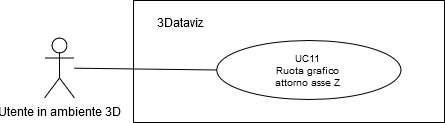
\includegraphics[scale=0.7]{template/images/UC11.png}
    \caption{UC11 - Selezione elementi}
\end{figure}
\begin{itemize}    
    \item \textbf{Attore:} utente;
    \item \textbf{Descrizione:} L'utente, tramite interazione opportuna, può selezionare una barra del grafico all'interno dell'ambiente 3D oppure una singola cella nella tabella.
    \item \textbf{Precondizioni:}    
        \begin{itemize}
            \item Il caricamento del dataset è avvenuto con successo;
            \item La generazione dell'ambiente 3D e del relativo grafico non hanno riscontrato errori;
            \item La generazione della tabella non ha riscontrato errori;
            \item Viene eseguita l'interazione opportuna da parte dell'utente per la selezione.
        \end{itemize}    
    \item \textbf{Postcondizioni:}
        \begin{itemize}
            \item Viene evidenziata la selezione.
        \end{itemize}    
    \item \textbf{Scenario:} 
        \begin{itemize}
            \item L'utente interagisce con l'ambiente 3D e seleziona una barra del grafico oppure seleziona una cella della tabella.
        \end{itemize}
\end{itemize}

\pagebreak

\subsubsection{UC11.1 - Selezione di un elemento del grafico}
\begin{figure}[h!]\centering
    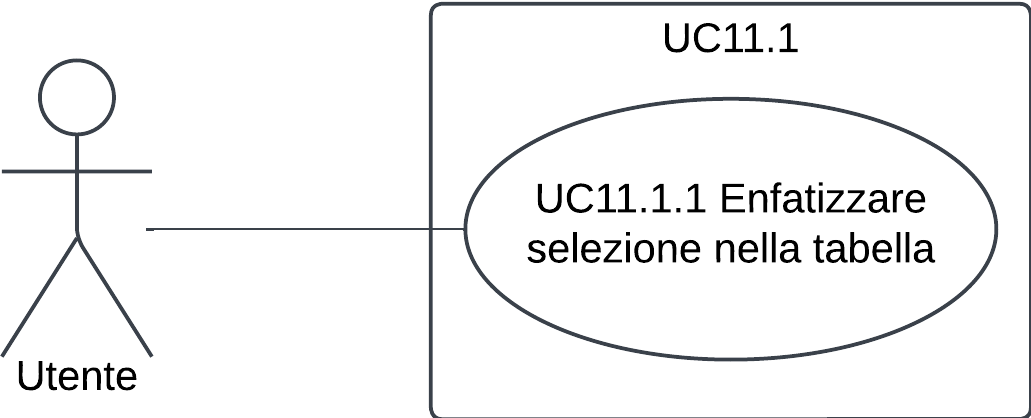
\includegraphics[scale=0.7]{template/images/UC11.1.png}
    \caption{UC11.1 - Selezione di un elemento del grafico}
\end{figure}
\begin{itemize}    
    \item \textbf{Attore:} utente;
    \item \textbf{Descrizione:} L'utente può selezionare una barra del grafico 3D.
    \item \textbf{Precondizioni:}    
        \begin{itemize}
            \item Il caricamento del dataset è avvenuto con successo;
            \item La generazione dell'ambiente 3D e del relativo grafico non hanno riscontrato errori;
            \item Viene eseguita l'interazione opportuna da parte dell'utente per la selezione.
        \end{itemize}    
    \item \textbf{Postcondizioni:}
        \begin{itemize}
            \item Viene evidenziata della barra del grafico 3D.
        \end{itemize}    
    \item \textbf{Scenario:} 
        \begin{itemize}
            \item L'utente interagisce con il grafico 3D e seleziona una barra.
        \end{itemize}
\end{itemize}
\paragraph{UC11.1.1 - Enfatizzazione della selezione nella tabella}
\begin{itemize}    
    \item \textbf{Attore:} utente;
    \item \textbf{Descrizione:} Viene evidenziata in maniera opportuna nella tabella la selezione compiuta dall'utente nel grafico 3D.
    \item \textbf{Precondizioni:}    
        \begin{itemize}
            \item Il caricamento del dataset è avvenuto con successo;
            \item La generazione della tabella non ha riscontrato errori;
            \item Viene eseguita l'interazione opportuna da parte dell'utente per la selezione.
        \end{itemize}    
    \item \textbf{Postcondizioni:}
        \begin{itemize}
            \item Viene evidenziata la cella nella tabella.
        \end{itemize}    
    \item \textbf{Scenario:} 
        \begin{itemize}
            \item L'utente interagisce con il grafico 3D, evidenziando la corrispondente cella della tabella.
        \end{itemize}
\end{itemize}

\pagebreak

\subsubsection{UC11.2 - Selezione di una cella della tabella}
\begin{figure}[h!]\centering
    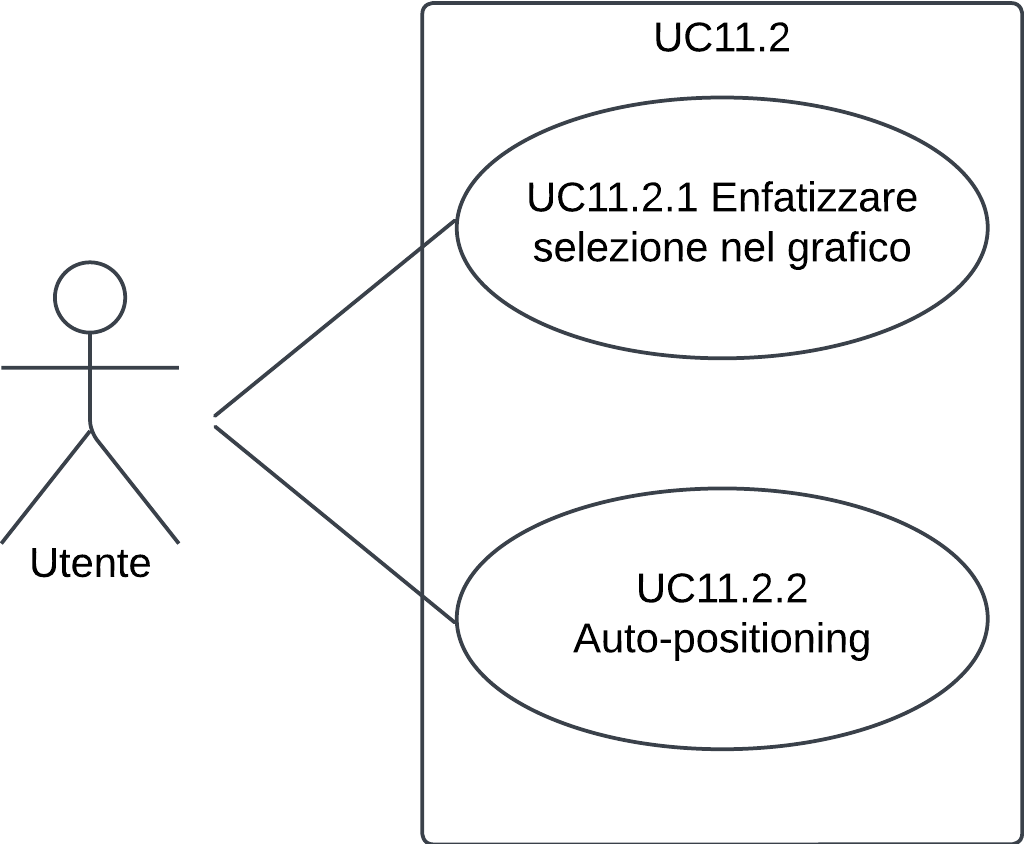
\includegraphics[scale=0.7]{template/images/UC11.2.png}
    \caption{UC11.2: Selezione di una cella della tabella}
\end{figure}
\begin{itemize}    
    \item \textbf{Attore:} utente;
    \item \textbf{Descrizione:} L'utente può selezionare una cella all'interno della tabella.
    \item \textbf{Precondizioni:}    
        \begin{itemize}
            \item Il caricamento del dataset è avvenuto con successo;
            \item La generazione della tabella non ha riscontrato errori;
            \item Viene eseguita l'interazione opportuna da parte dell'utente per la selezione della cella.
        \end{itemize}    
    \item \textbf{Postcondizioni:}
        \begin{itemize}
            \item Viene evidenziata la cella della tabella.
        \end{itemize}    
    \item \textbf{Scenario:} 
        \begin{itemize}
            \item L'utente interagisce con la tabella selezionando una cella la quale verrà evidenziata.
        \end{itemize}
\end{itemize}
\paragraph{UC11.2.1 - Enfatizzazione selezione nel grafico}
\begin{itemize}    
    \item \textbf{Attore:} utente;
    \item \textbf{Descrizione:} Viene evidenziata in maniera opportuna nel grafico 3D la selezione compiuta dall'utente nella tabella.
    \item \textbf{Precondizioni:}    
        \begin{itemize}
            \item Il caricamento del dataset è avvenuto con successo;
            \item La generazione dell'ambiente 3D e del relativo grafico non hanno riscontrato errori;
            \item Viene eseguita l'interazione opportuna da parte dell'utente per la selezione.
        \end{itemize}    
    \item \textbf{Postcondizioni:}
        \begin{itemize}
            \item Viene evidenziata la barra del grafico 3D.
        \end{itemize}    
    \item \textbf{Scenario:} 
        \begin{itemize}
            \item L'utente interagisce con una cella della tabella, evidenziando la corrispondente barra del grafico 3D.
        \end{itemize}
\end{itemize}
\paragraph{UC11.2.2 - Auto-positioning}
\begin{itemize}    
    \item \textbf{Attore:} utente;
    \item \textbf{Descrizione:} In seguito alla selezione di una cella, la vista si sposta sulla corrispondente barra del grafico 3D, centrandola sullo schermo.
    \item \textbf{Precondizioni:}    
        \begin{itemize}
            \item Il caricamento del dataset è avvenuto con successo;
            \item La generazione dell'ambiente 3D e del relativo grafico non hanno riscontrato errori;
            \item Viene richiesta un'operazione di auto-positioning.
        \end{itemize}    
    \item \textbf{Postcondizioni:}
        \begin{itemize}
            \item La telecamera e la relativa inquadratura saranno in una posizione diversa da quella iniziale e avranno inoltre in primo piano la barra selezionata del grafico 3D.
        \end{itemize}    
    \item \textbf{Scenario:} 
        \begin{itemize}
            \item L'utente seleziona una cella della tabella e la telecamera nell'ambiente 3D si sposta di conseguenza inquadrando la corrispettiva barra del grafico.
        \end{itemize}
\end{itemize}

\subsection{UC12 - Modifica trasparenza barra del grafico}
\begin{figure}[h!]\centering
    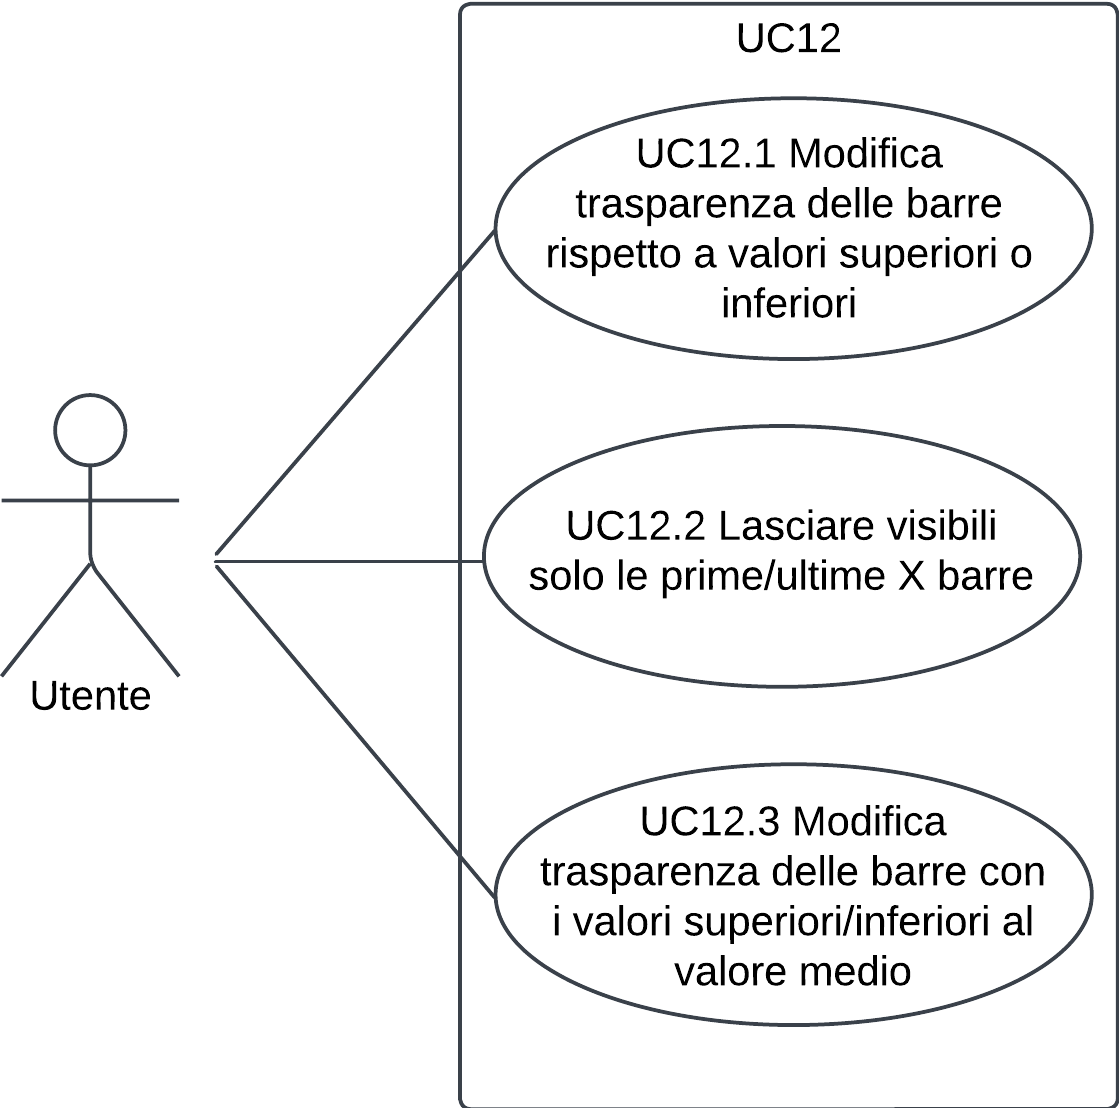
\includegraphics[scale=0.7]{template/images/UC12.png}
    \caption{Modifica trasparenza barra del grafico}
\end{figure}
\begin{itemize}    
    \item \textbf{Attore:} utente;
    \item \textbf{Descrizione:} Viene aumentata la trasparenza di una barra del grafico all'interno dell'ambiente 3D.
    \item \textbf{Precondizioni:}    
        \begin{itemize}
            \item Il caricamento del dataset è avvenuto con successo;
            \item La generazione dell'ambiente 3D e del relativo grafico non hanno riscontrato errori.
        \end{itemize}    
    \item \textbf{Postcondizioni:}
        \begin{itemize}
            \item Il valore di trasparenza delle altre barre del grafico 3D è maggiore rispetto a quello delle altre.
        \end{itemize}    
    \item \textbf{Scenario:} 
        \begin{itemize}
            \item L'utente evidenzia una determinata barra del grafico viene aumentato il valore di trasparenza a tutte le altre.
        \end{itemize}
\end{itemize}
\subsubsection{UC12.1 - Modifica trasparenza delle barre rispetto a valori superiori o inferiori}
\begin{itemize}    
    \item \textbf{Attore:} utente;
    \item \textbf{Descrizione:} L'utente può stabilire un valore limite al di sopra o al di sotto del quale alcune barre verranno evidenziate.
    \item \textbf{Precondizioni:}    
        \begin{itemize}
            \item Il caricamento del dataset è avvenuto con successo;
            \item La generazione dell'ambiente 3D e del relativo grafico non hanno riscontrato errori;
            \item La generazione dell'interfaccia non ha riscontrato errori;
            \item L'utente imposta correttamente tutti i parametri necessari.
        \end{itemize}    
    \item \textbf{Postcondizioni:}
        \begin{itemize}
            \item Ogni barra selezionata nel grafico 3D viene resa più visibile rendendo le altre barre più trasparenti.
        \end{itemize}    
    \item \textbf{Scenario:} 
        \begin{itemize}
            \item L'utente interagisce con l'interfaccia selezionando il numero di barre con i valori più elevati o più bassi da evidenziare nel grafico 3D.
        \end{itemize}
\end{itemize}
\subsubsection{UC12.2 - Lasciare visibili solo le prime/ultime X barre}
\begin{itemize}    
    \item \textbf{Attore:} utente;
    \item \textbf{Descrizione:} L'utente può selezionare quante barre con i valori più elevati o più bassi evidenziare.
    \item \textbf{Precondizioni:}    
        \begin{itemize}
            \item Il caricamento del dataset è avvenuto con successo;
            \item La generazione dell'ambiente 3D e del relativo grafico non hanno riscontrato errori;
            \item La generazione dell'interfaccia non ha riscontrato errori;
            \item L'utente imposta correttamente tutti i parametri necessari.
        \end{itemize}    
    \item \textbf{Postcondizioni:}
        \begin{itemize}
            \item Ogni barra selezionata nel grafico 3D viene resa più visibile rendendo le altre barre più trasparenti.
        \end{itemize}    
    \item \textbf{Scenario:} 
        \begin{itemize}
            \item L'utente interagisce con l'interfaccia selezionando il numero di barre con i valori più elevati o più bassi da evidenziare nel grafico 3D.
        \end{itemize}
\end{itemize}
\subsubsection{UC12.3 - Modifica trasparenza delle barre con i valori superiori/inferiori al valore medio}
\begin{itemize}    
    \item \textbf{Attore:} utente;
    \item \textbf{Descrizione:} L'utente può scegliere se evidenziare nel grafico 3D le barre il quale valore è superiore o inferiore al valore medio.
    \item \textbf{Precondizioni:}    
        \begin{itemize}
            \item Il caricamento del dataset è avvenuto con successo;
            \item La generazione dell'ambiente 3D e del relativo grafico non hanno riscontrato errori;
            \item La generazione dell'interfaccia non ha riscontrato errori;
            \item L'utente imposta correttamente tutti i parametri necessari.
        \end{itemize}    
    \item \textbf{Postcondizioni:}
        \begin{itemize}
            \item Ogni barra con il rispettivo valore superiore/inferiore al valore medio verrà opacizzata.
        \end{itemize}    
    \item \textbf{Scenario:} 
        \begin{itemize}
            \item L'utente interagisce con l'interfaccia per evidenziare nel grafico 3D solo le barre con un valore superiore o inferiore al valore medio.
        \end{itemize}
\end{itemize}

\subsection{UC13 - Visualizzazione di un piano parallelo alla base}
\begin{figure}[h!]\centering
    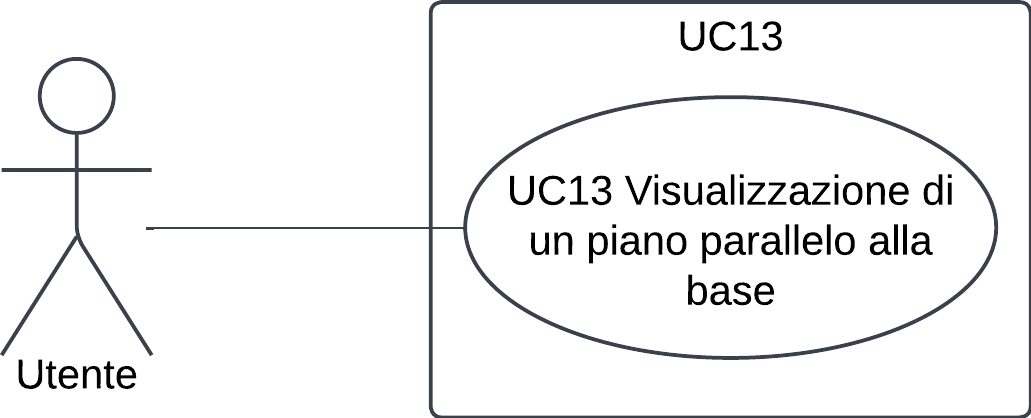
\includegraphics[scale=0.7]{template/images/UC13.png}
    \caption{UC13 - Visualizzazione di un piano parallelo alla base}
\end{figure}
\begin{itemize}    
    \item \textbf{Attore:} utente;
    \item \textbf{Descrizione:} Un piano, parallelo alla base, viene inserito nel grafico 3D per evidenziare un valore di interesse, scelto dall'utente tra quelli ricavabili dai dati. Questo piano offre una rappresentazione visiva immediata del valore selezionato.
    \item \textbf{Precondizioni:}    
        \begin{itemize}
            \item Il caricamento del dataset è avvenuto con successo;
            \item La generazione dell'ambiente 3D e del relativo grafico non hanno riscontrato errori.
        \end{itemize}    
    \item \textbf{Postcondizioni:}
        \begin{itemize}
            \item Viene generato un piano, nel grafico 3D, parallelo alla base che evidenzia il valore di interesse scelto dall'utente.
        \end{itemize}    
    \item \textbf{Scenario:} 
        \begin{itemize}
            \item L'utente può evidenziare un determinato valore di interesse (ad esempio il valore medio) ed esso sarà rappresentato nel grafico dal piano generato.
        \end{itemize}
\end{itemize}

\pagebreak

\subsection{UC14 - Visualizzazione errore nel caricamento del dataset}
\begin{figure}[h!]\centering
    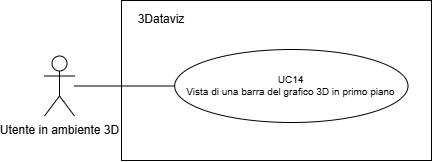
\includegraphics[scale=0.7]{template/images/UC14.png}
    \caption{UC14: Visualizzazione errore nel caricamento del dataset}
\end{figure}
\begin{itemize}    
    \item \textbf{Attore:} utente;
    \item \textbf{Descrizione:} L'utente visualizza un messaggio di errore dovuto al caricamento del dataset.
    \item \textbf{Precondizioni:}    
        \begin{itemize}
            \item L'utente ha selezionato il dataset da caricare;
            \item Il caricamento del dataset non è andato a buon fine.
        \end{itemize}    
    \item \textbf{Postcondizioni:}
        \begin{itemize}
            \item Viene visualizzato a schermo un messaggio di errore in seguito ad uno o più problemi riscontrati durante il caricamento del dataset selezionato.
        \end{itemize}    
    \item \textbf{Scenario:} 
        \begin{itemize}
            \item L'utente, in seguito al fallimento del caricamento del dataset selezionato, visualizza il messaggio di errore.
        \end{itemize}
\end{itemize}
